\documentclass[10pt, pdf, hyperref={unicode}]{beamer}

\usepackage[T2A]{fontenc}
\usepackage[utf8]{inputenc}
\usepackage[english, russian]{babel}
\usepackage{csquotes}
\usepackage{url}
\usepackage{indentfirst}
\usepackage{cmap} % чтобы работал поиск по PDF

\usepackage{tikz}
\usetikzlibrary{arrows.meta,shapes.arrows}
\usetikzlibrary{positioning}


\usepackage{amsmath}
\usepackage{amsfonts}
\usepackage{amssymb}
\usepackage{amsthm}
\usepackage{cmap} % чтобы работал поиск по PDF
\usepackage{graphicx}
\pdfcompresslevel=9
\usepackage{subcaption}


%\usepackage[usenames]{color}
%\usepackage{color}
%\usepackage{colortbl}


%\usepackage{tocloft}
%\usepackage{titlesec}

\usetheme{Madrid}

\makeatother
\author{Киселев Владимир}
\title[Анализ активности ЧД]{Анализ активности аккрецирующих рентгеновских пульсаров и черных дыр}
\institute[ФТШ]{Академический лицей <<Физико-техническая школа>>}
\date{}
%\titlegraphic{
\includegraphics[height=1cm,width=2cm]{pths_logo.png}}
%\titlegraphicii{
\includegraphics[height=1cm,width=2cm]{ioffe_logo.jpg}}
%\logo{%
%	
\includegraphics[height=1.5cm,width=1cm]{pths_logo.png}~%
%	
\includegraphics[height=1cm,width=1cm]{ioffe_logo.jpg}%
%}

\begin{document}

	\setlength{\unitlength}{\textwidth}  % measure in textwidths

	\begin{frame}[plain]

		\maketitle
		
		\footnotesize
		\begin{tabular}[t]{@{}l@{\hspace{3pt}}p{.3\textwidth}@{}}
			Научный руководитель: Свинкин Дмитрий Сергеевич \\
			\\
			Место прохождения практики: \\ 
			
			Физико-технический институт имени А. Ф. Иоффе\\ 
			
			лаборатория экспериментальной астрофизики 
		\end{tabular}%

	\end{frame}
  	
	\begin{frame}
  	
		\frametitle{Нейтронные звезды}
  	
  		\begin{columns}[T]

  			\begin{column}{0.5\textwidth}
%  			\begin{block}{Схематическое строение}
  				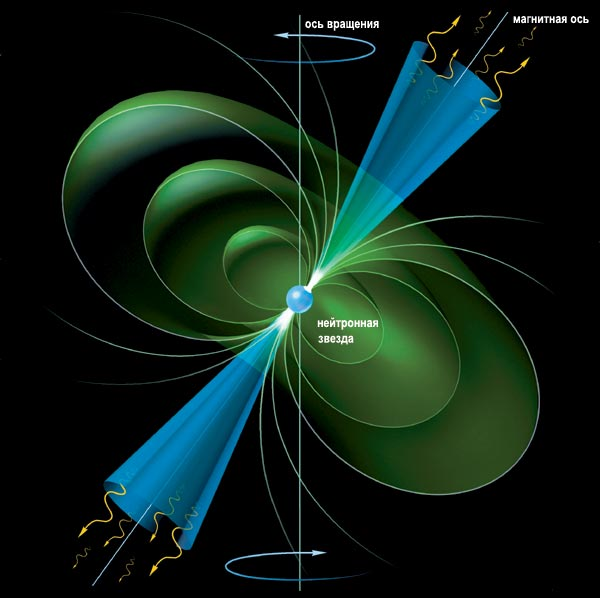
\includegraphics[width=\textwidth]{neutron_star}
%  			\end{block}
  			\end{column}
  	
  			\begin{column}{0.5\textwidth}
%  		  		\begin{block}{Особенности}
  		  		\begin{itemize}
  		  			\item Диаметр нейтронной звезды $\sim 10 \div 20$ км
  		  			\item $\overrightarrow{B} \sim 10^{12} \div 10^{13}$ Гс
  		  			\item образуется в результате коллапса ядра в воремя взрыва сверхновой
  		  			\item в начале своего жизненного цикла может соверщать около 100 оборотов в секунду
  		  			\item столь сильное магнитное поле и быстрое вращение --- причины рентгеновского вохникновения рентгеновского пульсара
  		  		\end{itemize}
%  		  		\end{block}
  			\end{column}
		\end{columns}
  	
	\end{frame}
  
	\begin{frame}
		
		\frametitle{Аккрецирующие рентгеновские пульсары}
		
		\begin{columns}[T]
			
			\begin{column}{0.7\textwidth}
				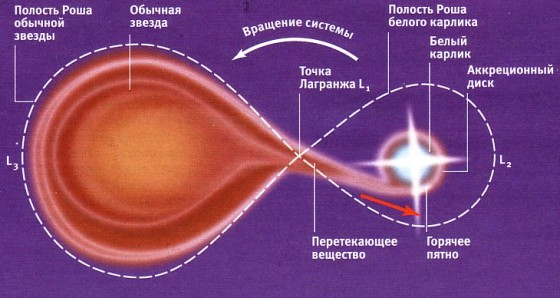
\includegraphics[width=\textwidth]{roche_lobe}
			\end{column}
			
			\begin{column}{0.3\textwidth}
				Полость Роша ---  область вокруг звезды, внешней границей которой служит поверхность равного потенциала, содержащая так называемую первую точку Лагранжа $L_{1}$.
			\end{column}
			
		\end{columns}
		
	\end{frame}

	\begin{frame}
		
		\frametitle{Черные дыры и рентгеновские пульсары}
		
		\begin{columns}[T]
			
			\begin{column}{0.5\textwidth}
				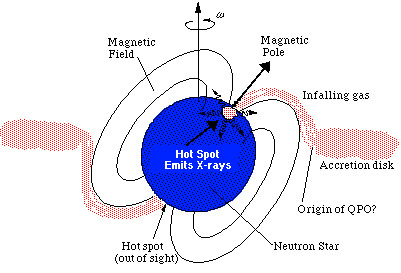
\includegraphics[width = \textwidth]{xray_pulsar.jpg}
			\end{column}
			
			\begin{column}{0.5\textwidth}
				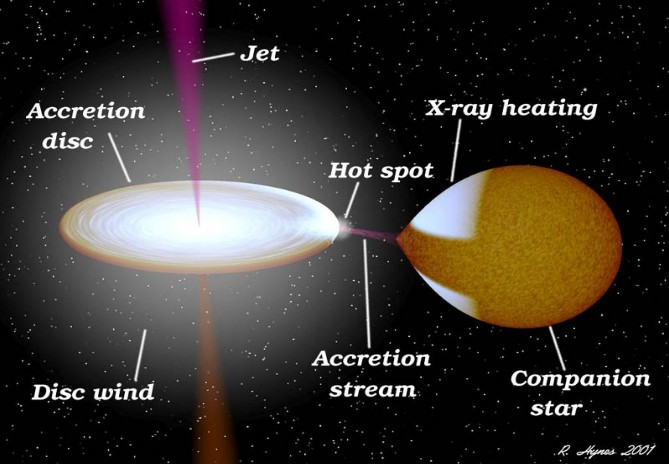
\includegraphics[width = \textwidth]{black_hole.jpg}
			\end{column}
		
		\end{columns}
		
	\end{frame}		

	\frame{
		\frametitle{Способы изучения источника}
		\par
		\begin{picture}(0.0, 1.0)
			\put(0.35, 0.35){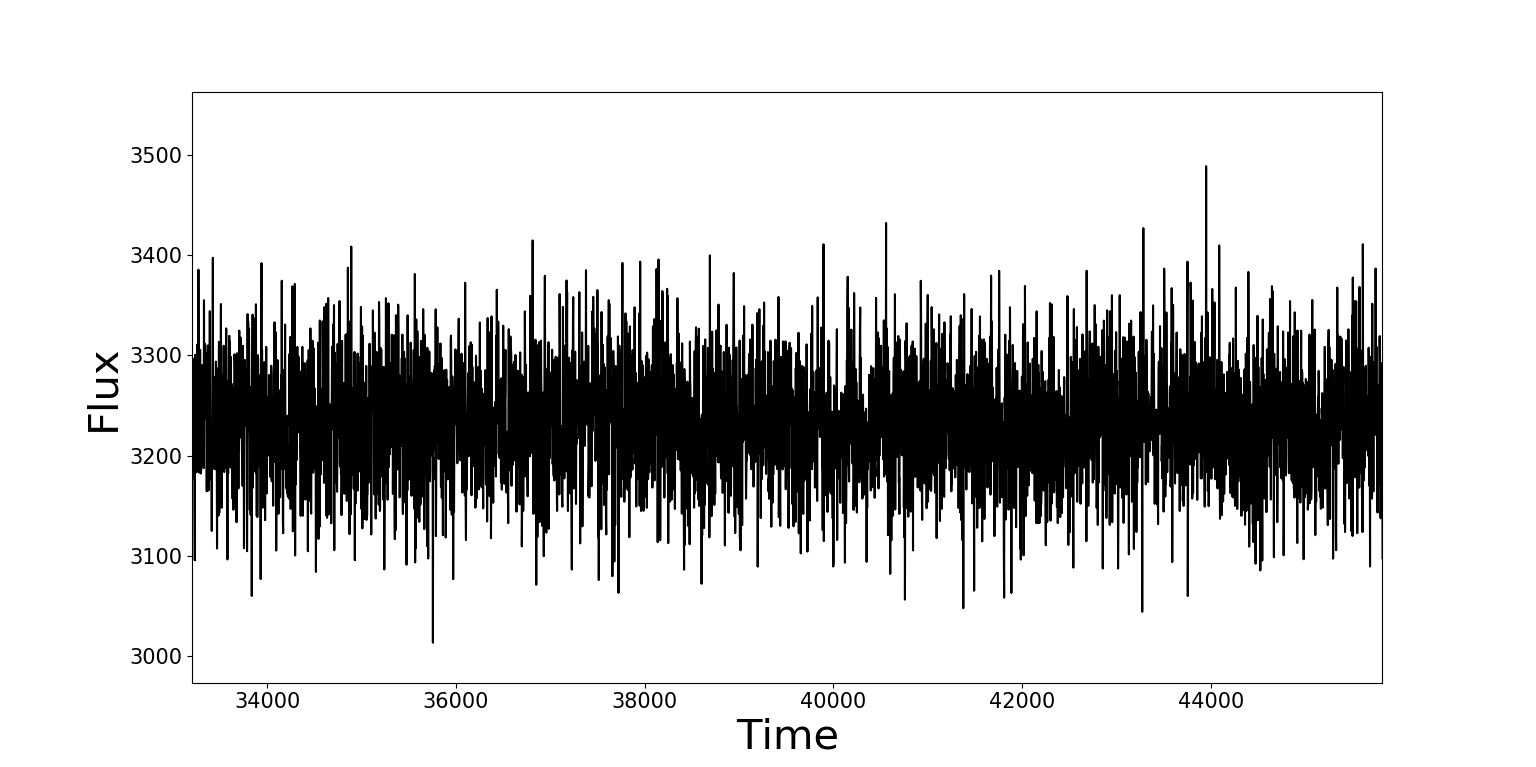
\includegraphics[width = 0.75\textwidth]{time-graph}}
			\put(0.0, 0.7){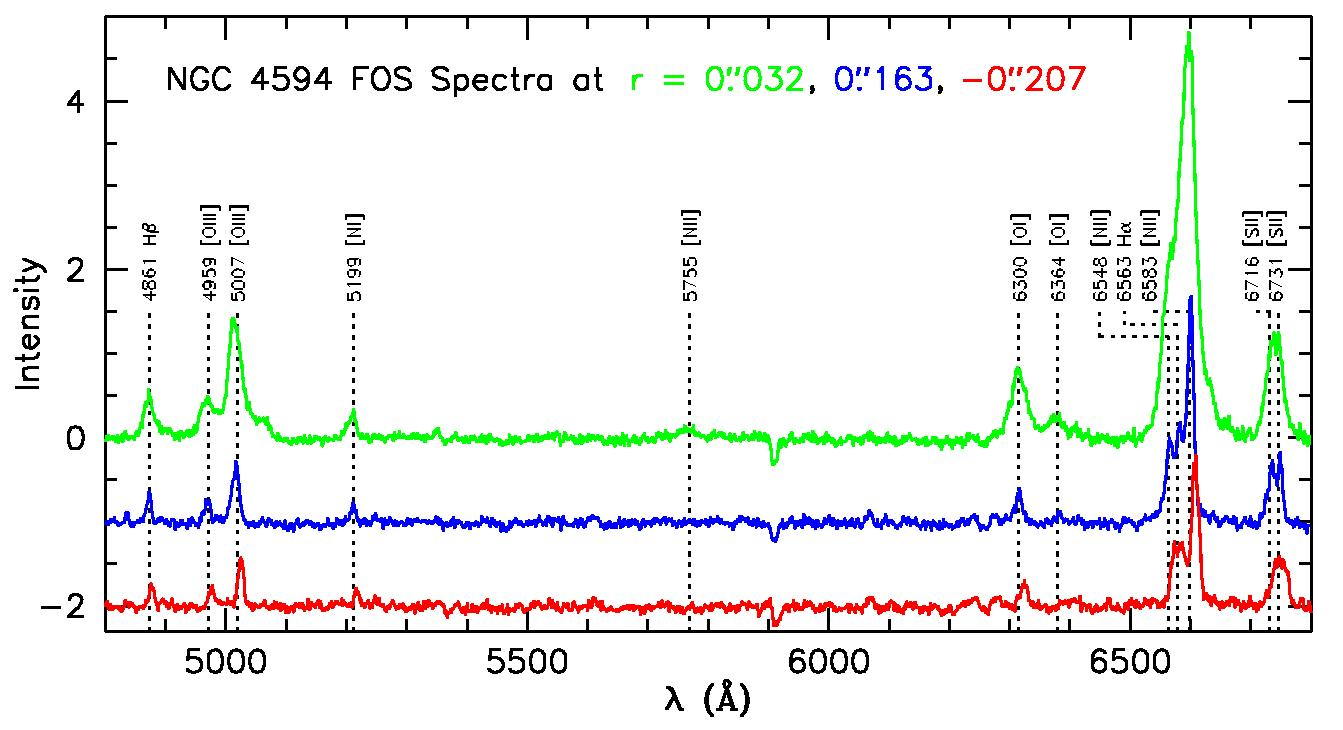
\includegraphics[width = 0.55\textwidth]{emission-spectrum}}
		\end{picture}
		\par
	}

	\begin{frame}
		\frametitle{Преобразование Фурье}

		\par
		\begin{picture}(0.0, 1.0)
			\put(0.35, 0.35){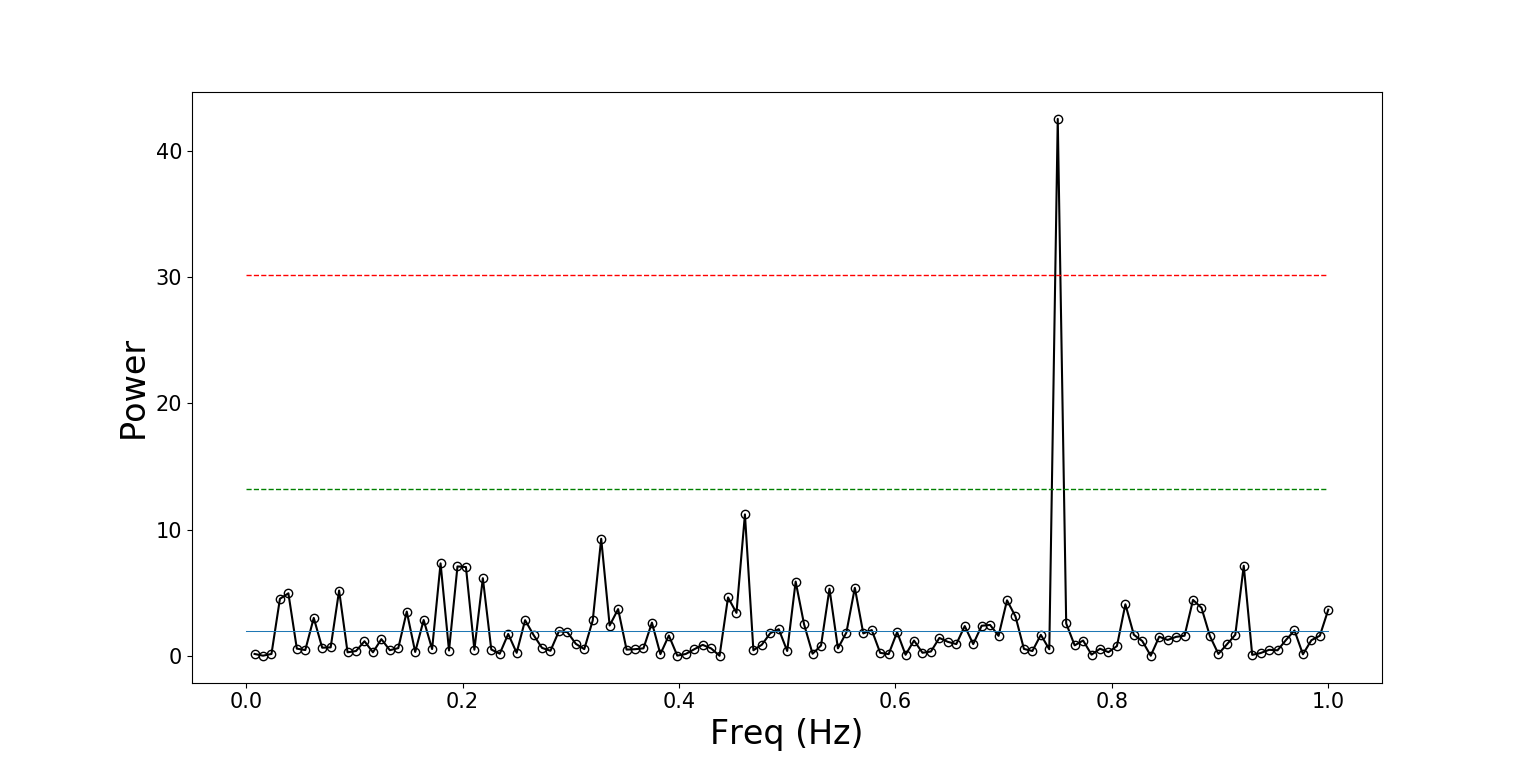
\includegraphics[width = 0.74\textwidth]{fourier}}
			\put(-0.05, 0.68){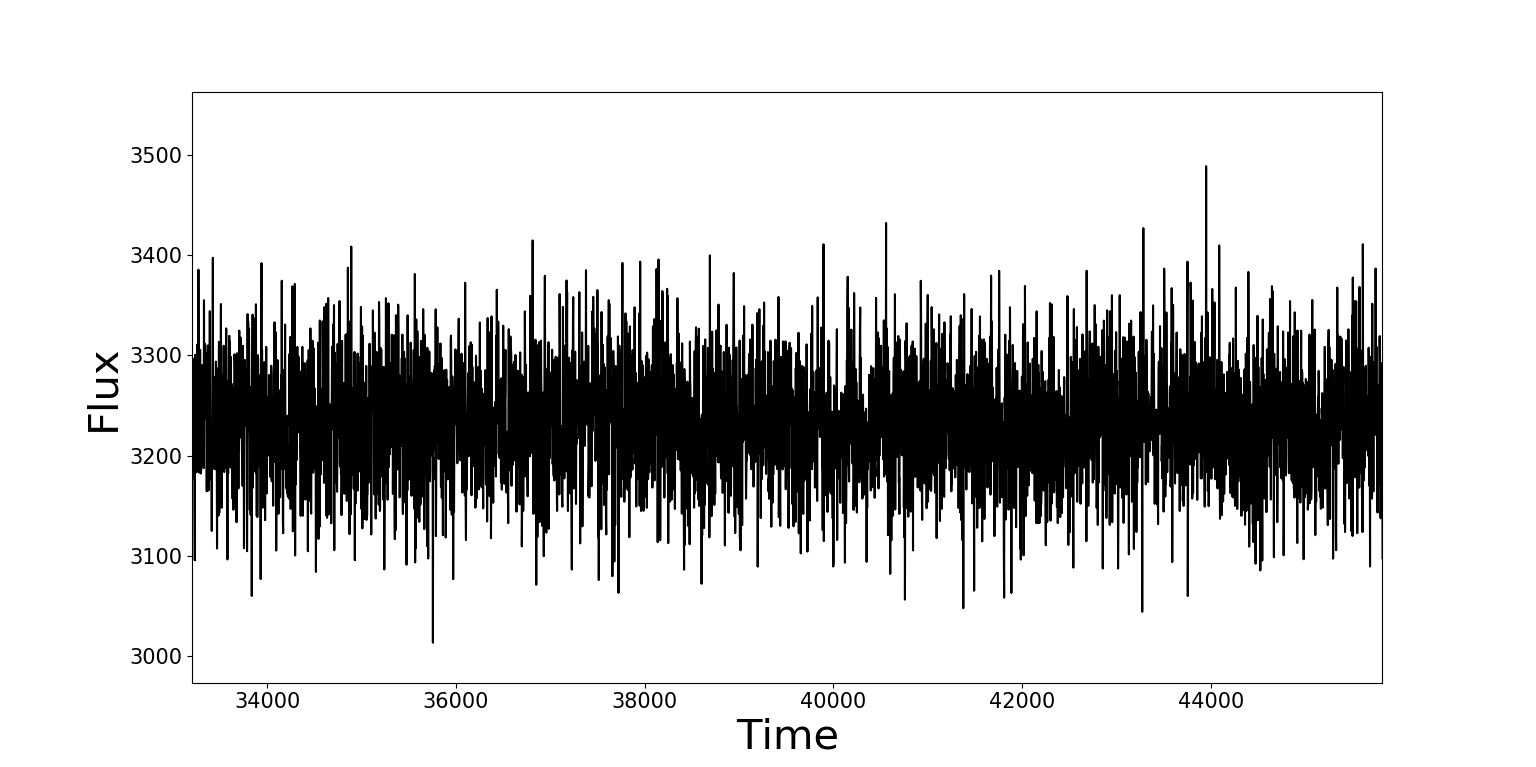
\includegraphics[width = 0.65\textwidth]{time-graph}}
		\end{picture}
		\par

	\end{frame}
	
	\begin{frame}
		\frametitle{Преобразование Фурье}
		
		Преобразованием Фурье функции $f(x)$ называется функция $\hat{f}(\omega)$ такая, что:		
		
		\begin{block}{}
			$$ \hat{f}(\omega) = \int\limits^{+\infty}_{-\infty} f(x) e^{-2 \pi i x \omega} \, \mathrm{d} x $$
		\end{block}
		
		\centering
		
		Но поскольку сигнал в реальности --- дискретный и конечный, то применяется дискретное преобразование Фурье, формула которого:
		
		\begin{block}{}
			$$ 	X_k = \sum^{N - 1}_{n = 0} x_n e^{-\frac{2 \pi i}{N} k n}, \text{где} $$
		\end{block}
		
		$x_n$ --- изначальный набор данных, $N$ ---	количество точек, в изначальном наборе данных, а $X_k$ --- набор данных, полученный после преобразования.

	\end{frame}

	\begin{frame}
	
		\frametitle{Цель работы}
		
		Кандидат в черную дыру MAXI J1820+070 был впервые зарегистрирован 11 марта 2018 года
		\begin{figure}
		\centering		
		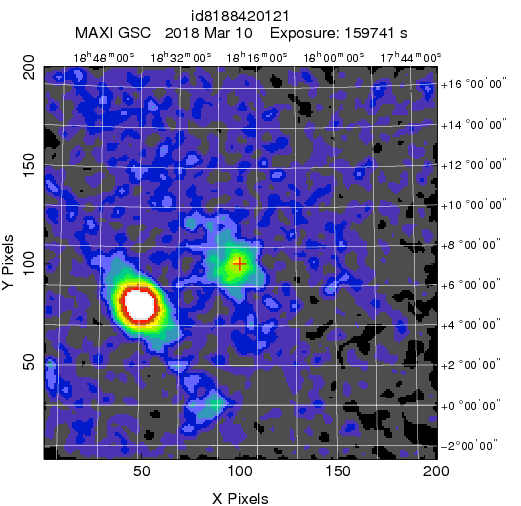
\includegraphics[width = 0.64\textwidth]{MAXI_J1820}
		\end{figure}
	
	\end{frame}
	
	\begin{frame}
	
		\frametitle{Квази-периодические осцилляции}
		
		\begin{figure}
		\centering
		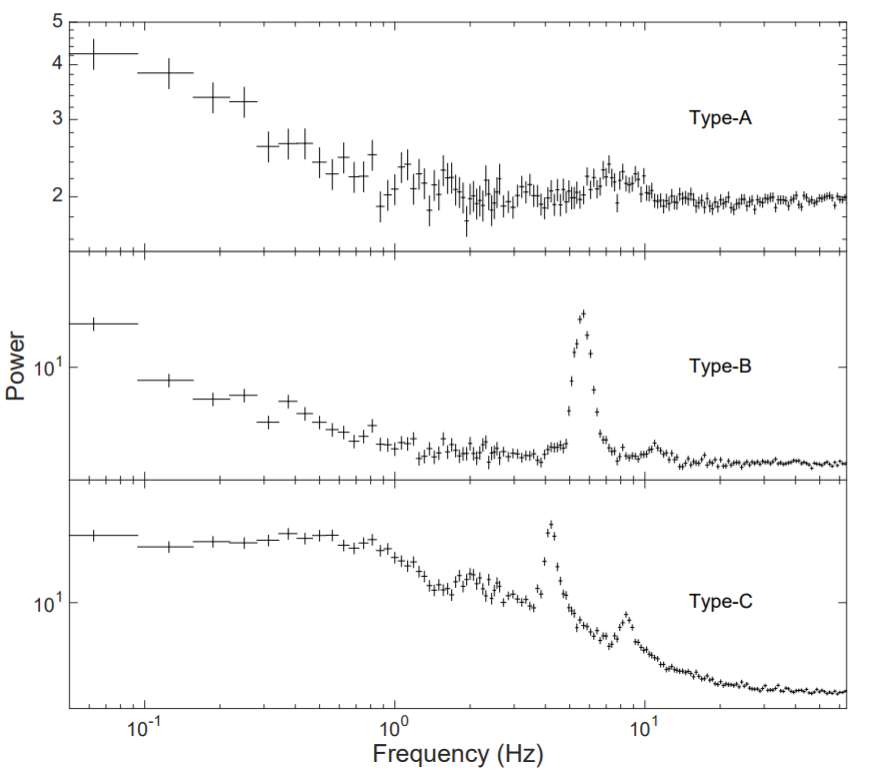
\includegraphics[width = 0.78\textwidth]{QPO}
		\end{figure}
	
	\end{frame}
	
	\begin{frame}
		
		\frametitle{Результаты}
		
		\begin{figure}
		\centering
		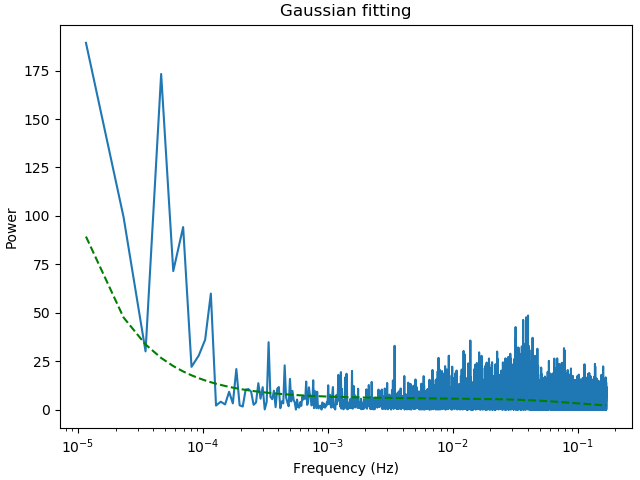
\includegraphics[width = 0.8\linewidth]{MAXI_J1820+070_KW_gaussian_approximation_day_41}
		\end{figure}
		
	\end{frame}
	
	\begin{frame}{}
  	\centering \Huge
  	\emph{Спасибо за внимание!}
	\end{frame}

	
\end{document}